\documentclass{beamer}

\usepackage{moy-slides}
\usepackage{tikz}
\usepackage{comment}

\title[Path-focusing]{Using bounded model checking to focus fixpoint iterations}

%\subtitle{} % (optional)

\author[Julien Henry]{Julien Henry}
% - Use the \inst{?} command only if the authors have different
%   affiliation.

\institute[Verimag]{Verimag (Grenoble INP)\\Grenoble\\France}

\tikzstyle{arrow}=[->,line width=.05cm,draw=red!90!blue!60!black]

% cf. Kevin
\tikzstyle{format}=[rectangle, draw,
top color=blue!25,bottom color=blue!60!black!25,shading=axis,shading angle=45,
drop shadow={shadow xshift=.75pt,shadow yshift=-.75pt}
]

\tikzstyle{phase}=[draw, line width=1pt, ellipse, inner sep=0pt,
font=\bfseries,
top color=white,bottom color=white!90!black,shading=axis,shading angle=45,
drop shadow={shadow xshift=.75pt,shadow yshift=-.75pt},
opacity=0.8]

\tikzstyle{arrowstyle}=[->, >=stealth', color=black, line width=0.7pt]
\tikzstyle{addon}=[circle, draw=red!15, fill=red!5, inner sep=0.3pt]

\usetikzlibrary{snakes,arrows,shapes,backgrounds,shadows,automata}
\usepgflibrary{snakes}

\tikzstyle{inline}=[remember picture,baseline,anchor=base,inner sep=0,outer sep=0,minimum height=0cm,minimum width=0, line width=0]
\tikzstyle{mycallout}=[
top color=yellow!7,bottom color=yellow!80!black!25,shading=axis,
% Cause display bug :-(
% shading angle=45,
ellipse callout, draw, drop shadow={shadow xshift=1pt,shadow yshift=-1pt}]

\date{March 22$^{th}$ 2011}

\begin{document}

\begin{frame}
  \titlepage
\end{frame}

\section[Introduction]{Introduction: Weakness of the standard approach}


\begin{frame}
  \frametitle{Example of standard Abstract Interpretation}

\begin{columns}
  \begin{column}{6cm}
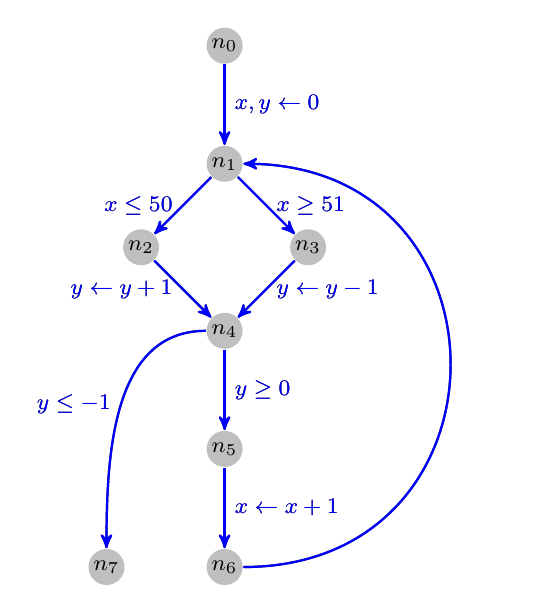
\begin{tikzpicture}[->,>=stealth',auto,node distance=1.5cm,
                    semithick,font=\footnotesize]
\tikzstyle{state}=[circle,fill=black!25,minimum size=13pt,inner sep=0pt]
\tikzstyle{transition}=[rectangle,thick,draw=black!75,
  			  fill=black!20,minimum size=4mm]
\tikzstyle{transition2}=[rectangle,thick,draw=blue!75,
  			  fill=blue!20,minimum size=4mm,blue]

	\node[state] (n0) {$n_0$};
	\node[state] (n1) [below of=n0] {$n_1$};
	\node[state] (n2) [below left of=n1] {$n_2$};
	\node[state] (n3) [below right of=n1] {$n_3$};
	\node[state] (n4) [below left of=n3] {$n_4$};
	\node[state] (n5) [below of=n4] {$n_5$};
	\node[state] (n6) [below of=n5] {$n_6$};
	\node[state] (n7) [left of=n6] {$n_7$};

	\node (n8) [right of=n6] {};
	\node (n9) [right of=n1] {};

  \path<-1> [transition] 
		(n0) edge              node {$x,y \leftarrow 0$} (n1);
  \path<-2> [transition] 
        (n1) edge			   node [left] {$x \leq 50$} (n2);
  \path<-7> [transition] 
        (n1)  edge              node [right] {$x \geq 51$} (n3);
  \path<-3> [transition] 
        (n2) edge              node [left] {$y \leftarrow y+1$} (n4);
  \path<-8> [transition] 
        (n3) edge			   node [right] {$y \leftarrow y-1$} (n4);
  \path<-4> [transition] 
        (n4) edge			   node {$y \geq 0$} (n5);
  \path<-10> [transition] 
		(n4) edge  [out = 180, in=90] node [left] {$y \leq -1$} (n7);
  \path<-5> [transition] 
        (n5) edge              node {$x \leftarrow x+1$} (n6);
  \path<-6> [transition] 
        (n6) edge [out=0, in=0, distance=3.5cm] node {} (n1);

  \path<2-> [transition2] 
		(n0) edge              node {$x,y \leftarrow 0$} (n1);
  \path<3-> [transition2] 
        (n1) edge			   node [left] {$x \leq 50$} (n2);
  \path<8-> [transition2] 
        (n1)  edge              node [right] {$x \geq 51$} (n3);
  \path<4-> [transition2] 
        (n2) edge              node [left] {$y \leftarrow y+1$} (n4);
  \path<9-> [transition2] 
        (n3) edge			   node [right] {$y \leftarrow y-1$} (n4);
  \path<5-> [transition2] 
        (n4) edge			   node {$y \geq 0$} (n5);
  \path<11-> [transition2] 
		(n4) edge  [out = 180, in=90] node [left] {$y \leq -1$} (n7);
  \path<6-> [transition2] 
        (n5) edge              node {$x \leftarrow x+1$} (n6);
  \path<7-> [transition2] 
        (n6) edge [out=0, in=0, distance=3.5cm] node {} (n1);
\end{tikzpicture}
\end{column}
\begin{column}{5cm}
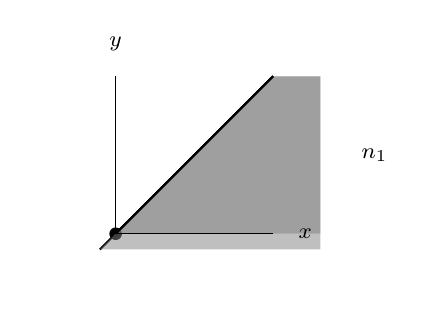
\begin{tikzpicture}[y=.2cm, x=.2cm,font=\footnotesize]
\tikzstyle{polyhedra}=[gray,opacity=0.5]
\tikzstyle{line}=[black,thick]

	\node (t1) at (-5,-4) {};
	\node (t2) at (13,11) {};
	\fill<2-6>[line] (0,0) circle (0.4);
	\draw<7-9>[line] (0,0) -- (10,10) -- cycle;
	\draw<10-11>[line] (-1,-1) -- (10,10) -- cycle;
	\fill<10-11>[polyhedra] (-1,-1) -- (10,10) -- (13,10) -- (13,-1) -- (0,-1) -- cycle;
	\fill<12-13>[polyhedra] (0,0) -- (10,10) -- (13,10) -- (13,0) -- cycle;
	\draw<12-13>[line] (0,0) -- (10,10) -- cycle;

 	%axis
	\draw (0,0) -- coordinate (x axis mid) (10,0);
    \draw (0,0) -- coordinate (y axis mid) (0,10);

	%ticks and labels      
	\node[right=1.2cm] at (x axis mid) {$x$};
	\node[above=1.2cm] at (y axis mid) {$y$};

	\node[right=3cm] at (y axis mid) {$n_1$};
\end{tikzpicture} 
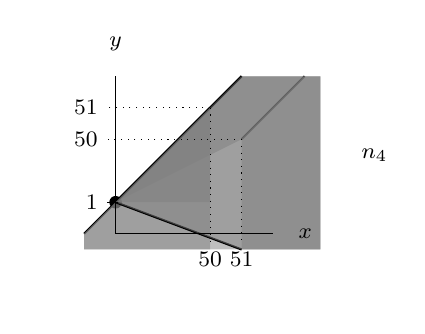
\begin{tikzpicture}[y=.2cm, x=.2cm,font=\footnotesize]
\tikzstyle{polyhedra}=[gray,opacity=0.5]
\tikzstyle{line}=[black,thick]

	\node (t1) at (-5,-4) {};
	\node (t2) at (13,11) {};
	\fill<4-8>[line] (0,2) circle (0.4);
	\fill<9-10>[polyhedra] (0,2) -- (8,10) -- (12,10) -- (8,6) --cycle;
	\draw<9-10>[line] (0,2) -- (6,8);
	\draw<9-10>[line] (8,6) -- (12,10);

	\draw<11-12>[line] (-2,0) -- (8,10);
	\fill<11-12>[polyhedra] (-2,-1) -- (-2,0) -- (8,10) -- (13,10) -- (13,-1) --
	 cycle;
	\fill<11-12>[polyhedra] (-2,-1) -- (-2,0) -- (6,8) -- (6,-1) -- cycle;
	\fill<11-13>[polyhedra] (8,6) -- (12,10) -- (13,10) -- (13,-1) -- (8,-1) -- cycle;

	\draw<13-13>[line] (0,2) -- (8,10);
	\draw<13-13>[line] (0,2) -- (8,-1);
	\fill<13-13>[polyhedra] (0,2) -- (8,10) -- (13,10) -- (13,-1) -- (8,-1) -- cycle;
	\fill<13-13>[polyhedra] (0,2) -- (6,8) -- (6,2) --  cycle;

 	%axis
	\draw (0,0) -- coordinate (x axis mid) (10,0);
    \draw (0,0) -- coordinate (y axis mid) (0,10);

	%labels      
	\node[right=1.2cm] at (x axis mid) {$x$};
	\node[above=1.2cm] at (y axis mid) {$y$};

	\node[right=3cm] at (y axis mid) {$n_4$};
	%ticks
     		\draw<4-13> (1pt,2) -- (-3pt,2) 
     			node[anchor=east] {1}; 
	
     		\draw<9-13> [dotted](6,8) -- (-3pt,8) 
     			node[anchor=east] {$51$}; 
     		\draw<9-13> [dotted] (8,6) -- (-3pt,6) 
     			node[anchor=east] {$50$}; 
     		\draw<9-13> [dotted](8,6) -- (8,-3pt) 
     			node[anchor=north] {$51$}; 
     		\draw<9-13> [dotted] (6,8) -- (6,-3pt) 
     			node[anchor=north] {$50$}; 
     		%\draw (2,1pt) -- (2,-3pt) 
     		%	node[anchor=north] {1}; 

\end{tikzpicture} 
\only<1-11>{Ascending iterations}
\only<12-13>{Descending iterations}
\end{column}
\end{columns}
\end{frame}

\begin{frame}
  \frametitle{Weakness of this approach}
yields imprecision when a loop has several phases.
\end{frame}

\begin{frame}
  \frametitle{My work}
\begin{enumerate}
\item Trying new methods to improve precision of the analysis.
\item Implementation of these methods, using:
\begin{itemize}
\item LLVM
\item Apron library
\item SMT-solvers like Yices, Z3\ldots
\end{itemize}
\item Make some experiments and trying to solve shotcomings.
\end{enumerate}
\end{frame}

\section[Lookahead Widening]{Lookahead Widening method}

\begin{frame}
  \frametitle{Principle}
\begin{itemize}
\item obtaining a solution for each loop phase before proceeding to the next.
\item widening \& narrowing at each loop phase.
\end{itemize}
\end{frame}

\begin{frame}
\frametitle{Example}
\end{frame}

\section[Path focusing]{Using SMT-solving to focus new paths}

\begin{frame}
  \frametitle{Principle}
\end{frame}

\begin{frame}
  \frametitle{Reducing the CFG}
\end{frame}

\begin{frame}
  \frametitle{using SMT-solving for finding new paths}
\end{frame}

\begin{frame}
  \frametitle{Example}
\end{frame}


\section[Work in progress]{Work in progress}

\begin{frame}
  \frametitle{What is done}
\begin{itemize}
\item a small analyzer, using LLVM and Apron
\item implementation of the Lookahead widening method
\item some tests
\end{itemize}
\end{frame}

\begin{frame}
  \frametitle{Work in progress}
\begin{itemize}
\item implementation of Path-focusing technique
\item experimental evaluation
\item How to compute $P_R$ ?
\end{itemize}
\end{frame}

\end{document}

%%% Local Variables:
%%% mode: latex
%%% TeX-master: t
%%% ispell-local-dictionary: "american"
%%% End:
